\chapter{Pipelining and Hazards}

Pipelining overlaps the execution of several instructions, like an assembly
line or doing laundry: while one load is in the dryer, the next is in the
washer. Each instruction still takes the same time (\emph{latency}), but
many more instructions complete per unit time (\emph{throughput}).

\section{The Five-Stage MIPS Pipeline}

\begin{center}
\begin{tabular}{lll}
\toprule
Stage & Name & Work \\
\midrule
IF & Instruction fetch & read IMem[PC], PC $\gets$ PC+4 \\
ID & Decode / register read & read registers, sign-extend, control \\
EX & Execute & ALU operation / address calculation \\
MEM & Memory & data memory read or write \\
WB & Write back & write result to register file \\
\bottomrule
\end{tabular}
\end{center}

Pipeline registers \textbf{IF/ID}, \textbf{ID/EX}, \textbf{EX/MEM},
\textbf{MEM/WB} separate the stages and carry all data and control signals
an instruction will need later (e.g.\ the destination register number must
travel all the way to WB).

\begin{figure}[H]
\centering
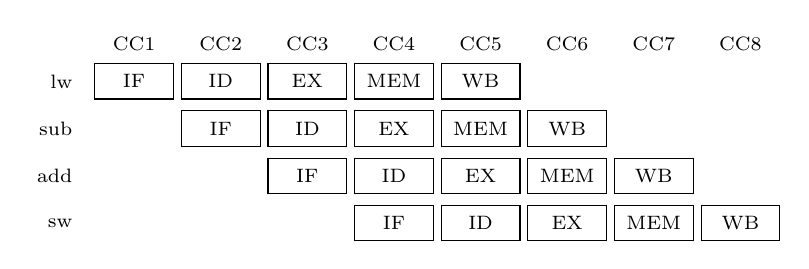
\begin{tikzpicture}[font=\scriptsize, x=1.1cm, y=0.6cm]
  \foreach \t in {1,...,8} \node at (\t,0.8) {CC\t};
  \foreach \i/\name in {0/lw, 1/sub, 2/add, 3/sw} {
    \node[anchor=east] at (0.4,-\i) {\code{\name}};
    \foreach \s/\lab in {0/IF,1/ID,2/EX,3/MEM,4/WB} {
      \pgfmathtruncatemacro{\c}{\i+\s+1}
      \node[draw, minimum width=1cm, minimum height=0.45cm] at (\c,-\i) {\lab};
    }
  }
\end{tikzpicture}
\caption{Pipeline diagram: four instructions overlap; one finishes every
cycle once the pipeline is full.}
\end{figure}

\subsection{Performance}

\begin{itemize}
  \item The clock period is set by the slowest \emph{stage} (plus pipeline
    register overhead).
  \item Ideal CPI $= 1$ (one instruction completes per cycle in steady state).
  \item $n$ instructions on a $k$-stage pipeline take $k + (n-1)$ cycles.
  \item Ideal speedup over an unpipelined design $\approx$ number of stages,
    if stages are balanced.
\end{itemize}

\begin{example}
Stage times 200, 100, 200, 200, 100\,ps. Single-cycle: 800\,ps per
instruction. Pipelined: clock 200\,ps. For 1\,000\,000 instructions:
single-cycle $8 \times 10^8$\,ps; pipelined $(5 + 999\,999) \times 200
\approx 2 \times 10^8$\,ps: speedup $\approx 4$, not 5, because the stages
are unbalanced.
\end{example}

MIPS is designed for pipelining: fixed-length instructions (easy fetch),
few formats with source registers in fixed positions (decode in parallel
with register read), memory operands only in loads/stores, aligned accesses.

\section{Hazards}

\begin{definition}
A \textbf{hazard} is a situation that prevents the next instruction from
executing in its scheduled cycle.
\begin{itemize}
  \item \textbf{Structural}: two instructions need the same hardware at once.
  \item \textbf{Data}: an instruction needs a value not yet produced.
  \item \textbf{Control}: the next instruction to fetch depends on a branch
    not yet resolved.
\end{itemize}
\end{definition}

\subsection{Structural hazards}

With a single memory, IF of one instruction and MEM of another would
conflict; MIPS avoids this with separate instruction and data memories
(caches). The register file is written in the first half of a cycle and
read in the second half, so WB and ID can share it.

\subsection{Data hazards}

\begin{lstlisting}[style=mips]
sub $2, $1, $3     # writes $2 in WB (cycle 5)
and $12, $2, $5    # reads $2 in ID (cycle 3)  -- hazard
or  $13, $6, $2    # reads $2 in cycle 4       -- hazard
add $14, $2, $2    # reads in cycle 5: OK (write first half, read second half)
sw  $15, 100($2)   # OK
\end{lstlisting}

These are \textbf{read-after-write (RAW)} dependences. Without help we would
need to \textbf{stall} (insert bubbles) for two cycles.

\paragraph{Forwarding (bypassing).} The result of \code{sub} exists at the
end of its EX stage, long before WB. A \textbf{forwarding unit} feeds it
directly from the EX/MEM or MEM/WB pipeline register into the ALU inputs.

\begin{important}[Forwarding conditions]
EX hazard (forward from EX/MEM):
\begin{center}
\code{EX/MEM.RegWrite} and \code{EX/MEM.Rd} $\ne 0$ and
\code{EX/MEM.Rd} = \code{ID/EX.Rs} (or \code{ID/EX.Rt}).
\end{center}
MEM hazard (forward from MEM/WB): same with MEM/WB, \emph{but only if} the
EX hazard condition does not also hold for that operand (the more recent
result wins).
\end{important}

\paragraph{Load-use hazard.} A loaded value is only available at the end of
MEM, so an instruction immediately using it cannot be helped by forwarding
alone:
\begin{lstlisting}[style=mips]
lw  $2, 20($1)
and $4, $2, $5     # needs $2 in EX, the same cycle lw is in MEM
\end{lstlisting}
The \textbf{hazard detection unit} in ID checks
\begin{center}
\code{ID/EX.MemRead} and (\code{ID/EX.Rt} = \code{IF/ID.Rs} or
\code{ID/EX.Rt} = \code{IF/ID.Rt})
\end{center}
and if true stalls one cycle: it prevents PC and IF/ID from updating and
zeroes the control signals going into ID/EX (a bubble, i.e.\ a \code{nop}).
After the one-cycle stall, forwarding from MEM/WB supplies the value.

\paragraph{Code scheduling.} The compiler can reorder instructions to avoid
load-use stalls.
\begin{example}
\lstinline[style=c]|a = b + e; c = b + f;|
\begin{lstlisting}[style=mips]
# original: 2 stalls          # reordered: 0 stalls
lw  $t1, 0($t0)               # lw  $t1, 0($t0)
lw  $t2, 4($t0)               # lw  $t2, 4($t0)
add $t3, $t1, $t2  # stall    # lw  $t4, 8($t0)
sw  $t3, 12($t0)              # add $t3, $t1, $t2
lw  $t4, 8($t0)               # sw  $t3, 12($t0)
add $t5, $t1, $t4  # stall    # add $t5, $t1, $t4
sw  $t5, 16($t0)              # sw  $t5, 16($t0)
\end{lstlisting}
\end{example}

\paragraph{Other dependences.} Write-after-read (WAR) and write-after-write
(WAW) cannot cause hazards in the simple in-order 5-stage pipeline (all
reads in ID, all writes in WB, in order) but matter in out-of-order
processors.

\subsection{Control hazards}

A \code{beq}'s outcome is known only after comparing registers. If resolved
in MEM (as in the basic design), three instructions have already been
fetched.

Approaches:
\begin{enumerate}
  \item \textbf{Stall} until the branch resolves (simple, slow).
  \item \textbf{Resolve earlier}: move the comparison (an XOR-based equality
    tester) and target adder into ID, so only one instruction is fetched
    behind the branch. This may itself require forwarding into ID and
    stalls if the branch's operand is being computed just before it.
  \item \textbf{Predict not taken}: keep fetching sequentially; if the branch
    is taken, \textbf{flush} the wrongly fetched instructions (turn them into
    nops).
  \item \textbf{Delayed branch} (classic MIPS): the instruction right after
    the branch (the \emph{delay slot}) always executes; the compiler fills
    it with useful work or a \code{nop}.
  \item \textbf{Dynamic branch prediction}: hardware remembers past
    behaviour.
\end{enumerate}

\paragraph{Dynamic prediction.} A \textbf{branch history table} (branch
prediction buffer) is indexed by low bits of the branch address.
\begin{itemize}
  \item 1-bit predictor: remember the last outcome. A loop branch is
    mispredicted twice per execution of the loop (last iteration and first
    iteration next time).
  \item 2-bit saturating counter: change the prediction only after two
    consecutive mispredictions. A loop branch mispredicts once per loop.
  \item A \textbf{branch target buffer} caches target addresses so the
    target can be fetched in the next cycle.
\end{itemize}

\begin{figure}[H]
\centering
\begin{tikzpicture}[->, >=Stealth, thick, node distance=2.6cm, font=\scriptsize,
  every state/.style={minimum size=1.2cm, align=center}]
  \node[state] (st) {Strongly\\taken};
  \node[state, right of=st] (wt) {Weakly\\taken};
  \node[state, right of=wt] (wn) {Weakly\\not};
  \node[state, right of=wn] (sn) {Strongly\\not};
  \path (st) edge[loop above] node{T} (st)
        (st) edge[bend left] node[above]{N} (wt)
        (wt) edge[bend left] node[below]{T} (st)
        (wt) edge[bend left] node[above]{N} (wn)
        (wn) edge[bend left] node[below]{T} (wt)
        (wn) edge[bend left] node[above]{N} (sn)
        (sn) edge[bend left] node[below]{T} (wn)
        (sn) edge[loop above] node{N} (sn);
\end{tikzpicture}
\caption{2-bit saturating-counter branch predictor (T = taken, N = not taken).}
\end{figure}

\begin{example}[CPI with hazards]
Base CPI 1. 20\% of instructions are loads, half of which are followed by a
dependent instruction (1-cycle stall). 15\% are branches, predicted
not-taken, 60\% taken, penalty 1 cycle when mispredicted.
\[
\text{CPI} = 1 + 0.20 \times 0.5 \times 1 + 0.15 \times 0.6 \times 1 = 1.19.
\]
\end{example}

\section{Beyond the Basic Pipeline}

\begin{itemize}
  \item \textbf{Deeper pipelines} (superpipelining): more, shorter stages,
    higher clock rate, but larger branch penalties.
  \item \textbf{Multiple issue}: issue several instructions per cycle.
    \emph{Static} (VLIW: compiler bundles instructions) or \emph{dynamic}
    (superscalar: hardware decides). Then CPI $< 1$; we talk about IPC.
  \item \textbf{Out-of-order execution} with register renaming removes
    WAR/WAW false dependences and hides latencies; results are committed in
    order via a reorder buffer.
  \item \textbf{Exceptions} in a pipeline: flush the faulting instruction and
    those after it, save its PC in EPC, fetch from the handler.
\end{itemize}

\section*{Summary}
\begin{itemize}
  \item Five stages IF, ID, EX, MEM, WB with pipeline registers between them;
    ideal CPI 1, clock set by slowest stage, speedup $\le$ number of stages.
  \item Structural hazards: avoided by separate I/D memories and split-cycle
    register file.
  \item Data hazards: forwarding from EX/MEM and MEM/WB; load-use needs a
    1-cycle stall (hazard detection unit); compiler scheduling helps.
  \item Control hazards: stall, early resolution in ID, predict not taken
    with flush, delay slots, dynamic prediction (2-bit counters, BTB).
  \item CPI = 1 + stall cycles per instruction.
\end{itemize}
